\documentclass{VUMIFPSkursinis}
\usepackage{float}
\usepackage{hyperref}
\usepackage{algorithmicx}
\usepackage{algorithm}
\usepackage{algpseudocode}
\usepackage{amsfonts}
\usepackage{amsmath}
\usepackage{bm}
\usepackage{caption}
\usepackage{color}
\usepackage{graphicx}
\usepackage{listings}
\usepackage{subcaption}
\usepackage{wrapfig}
\usepackage{biblatex}
\usepackage{microtype}

\renewcommand\lstlistingname{Kodas}

% Titulinio aprašas
\university{Vilniaus universitetas}
\faculty{Matematikos ir informatikos fakultetas}
\institute{Informatikos institutas}  % Užkomentavus šią eilutę - institutas neįtraukiamas į titulinį
\department{Informatika}
\papertype{Referatas}
\title{Žinių grafikų užklausa naudojant užklausų kalbą SPARQL}
\titleineng{Querying knowledge graphs using query language SPARQL}
\status{2 kurso 1 grupės studentas}
\author{Tomas Kozakas}
% \secondauthor{Vardonis Pavardonis}   % Pridėti antrą autorių
\supervisor{Doc. Dr. Haroldas Giedra}
% \addsignatureplaces{} % prideda parašų vietas tituliniame puslapyje
\date{Vilnius – \the\year}

\bibliography{bibliografija}

\begin{document}
\maketitle

\tableofcontents

\sectionnonum{Įvadas}
Ne paslaptis, kad kai kurių projektų sėkmė praeityje buvo pagrįsta greitai ir stabiliai veikiančiomis paslaugomis. Pavyzdžiui, „Facebook“ draugų ratas buvo įgyvendintas naudojant grafus ir algoritmus, leidžiančius greitai rasti ir rodyti vartotojų tarpusavio ryšius. Informacijos paieškos efektyvumas yra neatsiejama kasdienio gyvenimo dalis. Populiariausia paieškos sistema „Google“ paieškos sistema irgi naudoja žinių grafais, tam kad efektyviai ir greitai pateikti mums aktualia informacija. Žinių grafikai yra labai naudinga technologija, tačiau norint iš jų gauti reikiamą informaciją, reikia turėti efektyvias užklausų sistemas. SPARQL yra viena iš tokių užklausos kalbų. Mano darbo tikslas yra išanalizuoti žinių grafų užklausų formavimą ir vykdymą naudojant tokia užklausų kalbą kaip SPARQL.

Siekiant šio tikslo, darbe bus atliekami keli etapai, kurie apims žinių grafų apibrėžimą ir pritaikymo analizę, SPARQL užklausų kalbos apžvalgą, SPARQL užklausų formavimo žinių grafams ir įvairių tipų užklausų pavyzdžių aptarimą, taip pat pavyzdinio žinių grafo analizę, įskaitant pavyzdinių užklausų formavimą ir analizę.

\section{Žinių grafų apibrėžimas}
Žinių grafų apibrėžimai gali skirtis. Pastraipa paremta tyrimu, vardu "Towards a Definition of Knowledge Graphs", kurios autoriai yra Lisa Ehrlinger ir Wolfram Wöß, pasiūlo įvairūs skirtingus apibrėžimus iš skirtingų autoritetingų šaltinių, vienas iš tokių apibrėžimų buvo pasiūlytas Semantic Web Company.
Pagal Semantic Web Company apibrėžimą žinių grafai gali būti apibrėžiami kaip visų tipų objektų tinklas, kuris yra esminis tam tikrai sričiai ar organizacijai. Jie neapsiriboja tik abstrakčiomis sąvokomis bei ryšiais, bet taip pat apima ir konkrečius elementus, tokius kaip dokumentai ar duomenų rinkiniai \cite{SemanticWebCompany}. Žinių grafai yra plačiai naudojami įvairiose pramonės šakose dėl jų sugebėjimo efektyviai analizuoti ir atskleisti tarpusavio ryšius tarp duomenų. Paieškos sistemose, pavyzdžiui, „Google“, žinių grafai padeda tobulinti paieškos rezultatus, pateikiant aktualią ir tikslesnę informaciją naudotojams. 

\subsection{Žinių grafų struktūra}
Pagal Stanfordo universitetą žinių grafas yra kryptinis grafas, kuriame taškų vardai turi aiškiai apibrėžtas reikšmes. Kryptinis grafas susideda iš taškų (nodes), briaunų (edges) ir taškų vardų. Taškai gali būti bet kas, pavyzdžiui, žmonės, įmonės, kompiuteriai ir t.t. Briauna (edge) jungia porą taškų (nodes) ir atspindi tarp jų dominančius ryšius, pavyzdžiui, draugystės ryšį tarp dviejų žmonių, kliento ryšį tarp įmonės ir asmens ar tinklo ryšį tarp dviejų kompiuterių. Taškų vardai užfiksuoja ryšio reikšmę, pavyzdžiui, draugystės ryšį tarp dviejų žmonių.\cite{stanford_what_2021}

\begin{figure}[htbp]
  \centering
  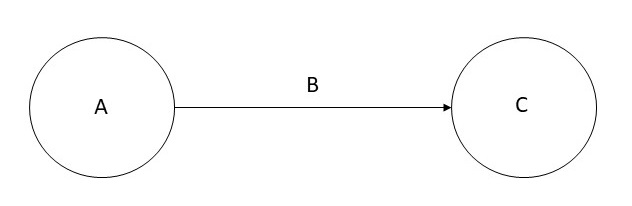
\includegraphics[width=0.5\textwidth]{img/triple.jpg}
  \caption{Grafo pavyzdis \cite{stanford_image}}
  \label{fig:sample_image}
\end{figure}
\pagebreak

 Pavyzdžiui, norint sukurti žinių grafą, panašų į Facebook draugų ratą, reikėtų:
\begin{enumerate}
\item Nurodyti žmones kaip taškus (galite nurodyti savo draugų vardus arba naudoti jų profilio nuotraukas kaip tašką):

\begin{figure}[htbp]
  \centering
  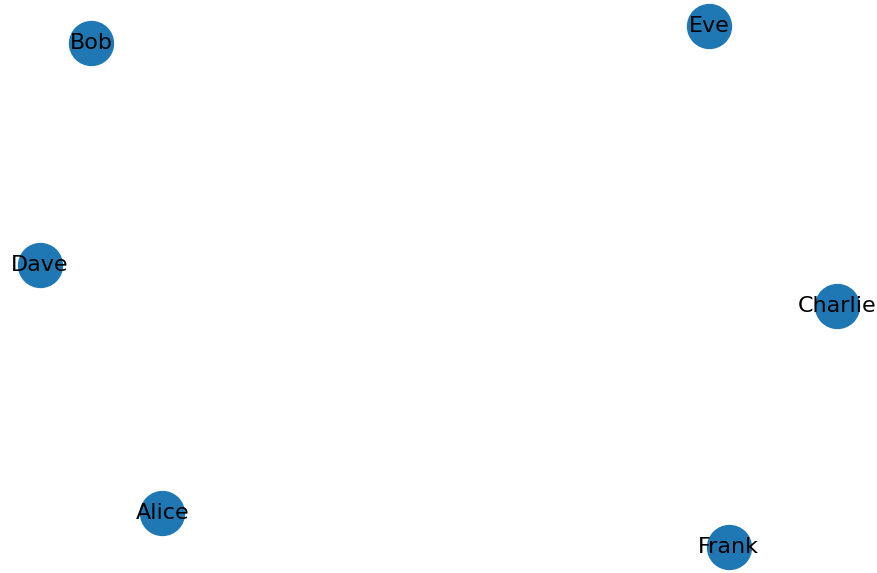
\includegraphics[width=0.7\textwidth]{img/nodes.png}
  \caption{Grafas, kur žmones reprezentuoja taškai}
  \label{fig:sample_image}
\end{figure}

\item Sukurti briaunas tarp draugų. Briaunos reprezentuos draugystes tarp žmonių. 
\begin{figure}[htbp]
  \centering
  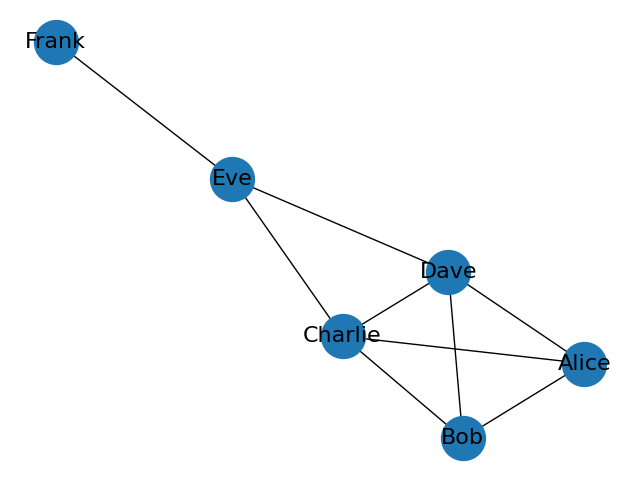
\includegraphics[width=0.6\textwidth]{img/vertex.png}
  \caption{Grafas, briaunos reprezentuos draugystes tarp žmonių}
  \label{fig:sample_image}
\end{figure}
\end{enumerate}

Matome, kaip "Alice" yra susietas su "Bob", "Charlie" ir "Dave", "Bob" yra susietas su "Charlie" ir "Dave", "Charlie" yra susietas su "Dave" ir "Eve", "Dave" yra susietas su "Eve", o "Eve" yra susietas su "Frank". Taip galime pridėti papildomų duomenų apie draugų santykius. Tai nėra žinių grafų riba ir galima parodyti daug informacijos, susijusios su žmonių draugų ratu, tokią kaip kada draugystė prasidėjo, kaip jie susipažino, kiek laiko jau draugauja ir t.t.

\pagebreak

\section{RDF modelio apibrėžimas}
Pagal Vikipediją Resource Description Framework (RDF) yra W3C sukurtas semantinio interneto standartas, skirtas struktūrizuotų metaduomenų aprašymui. RDF turi savo kalbą, RDF Schema (RDFS), ir semantikos aprašymą OWL \cite{wiki:rdf}. RDF grafas yra sudarytas iš trijų teiginių sakinio, pavadinto "triple", kuriame yra subjektas, predikatas ir objektas ir kiekvieną "triple" galima identifikuoti unikaliu URI. Pavyzdžiui, norint aprašyti, kad Vilnius yra Lietuvos sostinė, RDF triplas atrodytų taip:
\begin{enumerate}
    \item Subjektas: Vilnius
    \item Predikatas: yra sostinė
    \item Objektas: Lietuva
    
\end{enumerate}

\subsection{RDF modelis žinių grafų kūrimui}

Tarkime, turime RDR teiginius:
\begin{enumerate}
    \item Vilniaus yra Lietuvos sostine
    \item Lietuvos valiuta yra EUR
    \item Vilnius yra Vilniaus apskrities regionas
    \item Lietuvos gyventojų skaičius yra 2860002
    \item Vilniaus gyventojų skaičius yra 591632
    
\end{enumerate}

Kai identifikavom jų komponentus: subjektą, predikatą, ir objektą gaunam:
\begin{lstlisting}[captionpos=b, caption=Teiginio subjektas; predikatas ir objektas, label=lst:sparql, basicstyle=\ttfamily,frame=single]
    ("<Vilnius>", "<yra_sostine>", "<Lietuva>")
    ("<Lietuva>", "<valiuta>", "<EUR>"),
    ("<Vilnius>", "<regionas>", "<Vilniaus_apskritis>"),
    ("<Lietuva>", "<gyventoju_skaicius>", "<2860002>"),
    ("<Vilnius>", "<gyventoju_skaicius>", "<591632>")
\end{lstlisting}
\begin{lstlisting}[captionpos=b, caption=Teiginio RDF modelis, label=lst:sparql,
   basicstyle=\ttfamily,frame=single]
@prefix ex: <http://example.com/> .
@prefix rdf: <http://www.w3.org/1999/02/22-rdf-syntax-ns#> .

ex:Vilnius rdf:type rdf:Resource .
ex:Lietuva rdf:type rdf:Resource .
ex:EUR rdf:type rdf:Resource .
ex:VilniausApskritis rdf:type rdf:Resource .
ex:Vilnius ex:yraSostine ex:Lietuva .
ex:Lietuva ex:valiuta ex:EUR .
ex:Vilnius ex:regionas ex:VilniausApskritis .
ex:Lietuva ex:gyventojuSkaicius "2860002" .
ex:Vilnius ex:gyventojuSkaicius "591632" .

\end{lstlisting}

Kai identifikavom jų komponentus: subjektą, predikatą, ir objektą. Vaizduojame grafą, kur subjektas yra vieną viršūnė, objektas yra kitą viršūnė, o predikatas yra briauna, jungianti šias viršūnės:
\begin{figure}[htbp]
  \centering
  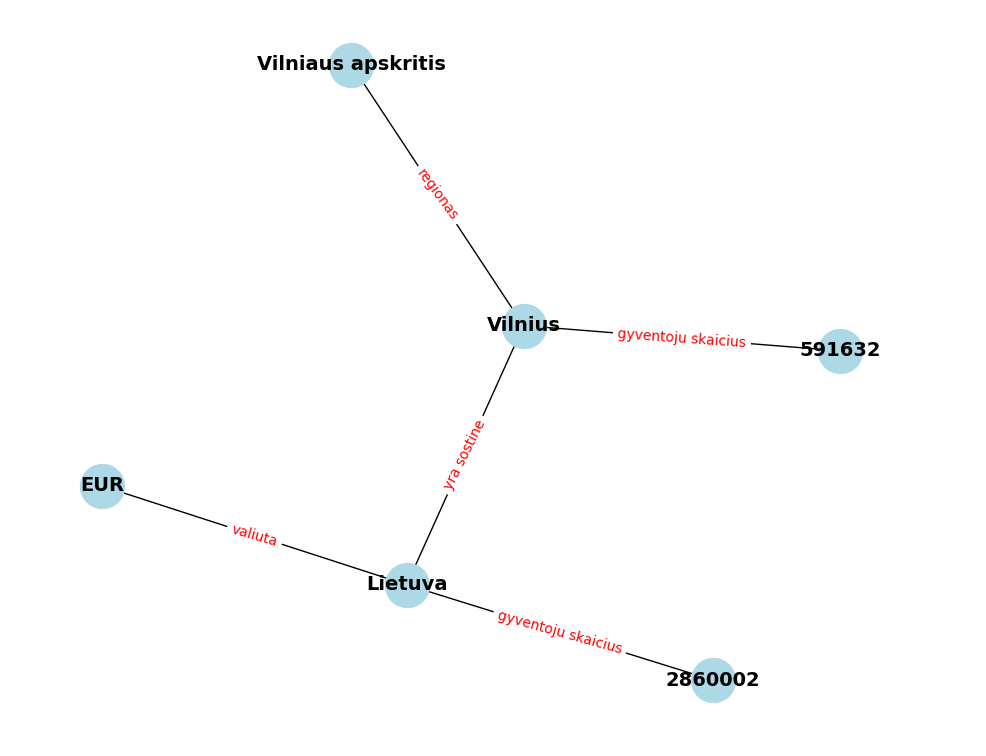
\includegraphics[width=1\textwidth]{img/rdf_example.png}
  \caption{Žinių grafas rdf modeliui}
  \label{fig:sample_image}
\end{figure}
\pagebreak

\section{SPARQL užklausų kalbos apžvalga}
Pagal Vikipedia RDF užklausų kalba, tai yra semantinė užklausų kalba duomenų bazių sistemoms, skirta gauti ir manipuliuoti duomenimis, saugomais RDF formatu \cite{wiki:sparql}.

Ši kalba suteikia daugybę galimybių ieškoti, filtruoti ir agreguoti duomenis, taip pat jungtis su kitais RDF duomenų šaltiniais. SPARQL matomi jūsų duomenys kaip nukreiptas, pažymėtas grafas, kuris viduje yra išreikštas kaip trijų elementų rinkiniai, sudaryti iš subjekto, predikato ir objekto.

\subsection{SPARQL pagrindai ir sintaksė}
SPARQL užklausų sintaksė yra panaši į SQL užklausų sintaksę, tačiau yra pritaikyta RDF duomenims ir palaiko daugybę semantinio tinklo operacijų. Pagrindinis grafų modelio šablonas sudarytas iš trijų elementų - subjekto, predikato ir objekto, kurie gali būti kintamieji (ženklas laukia reikšmės).

Pažvelkime į paprastą pavyzdį. Tarkime turime paprastą grafą kuris reprezentuoja žmonės ir jų adresai.
RDF elementai atrodytų taip:

\begin{lstlisting}[captionpos=b, caption=Žmonių RDF, label=lst:sparql,
   basicstyle=\ttfamily,frame=single]
<http://example.org/person1> ex:hasName "John" .
<http://example.org/person1> ex:hasAge 25 .
<http://example.org/person2> ex:hasName "Mary" .
<http://example.org/person2> ex:hasAge 30 .
<http://example.org/person3> ex:hasName "Peter" .
<http://example.org/person3> ex:hasAge 35 .
\end{lstlisting}

\begin{lstlisting}[captionpos=b, caption=Adresų rdf, label=lst:sparql,
   basicstyle=\ttfamily,frame=single]
<http://example.org/person1> ex:hasAddress "123 Main St" .
<http://example.org/person2> ex:hasAddress "456 Park Ave" .
<http://example.org/person3> ex:hasAddress "789 Elm St" .
\end{lstlisting}

Norėdami gauti informaciją apie žmones ir jų adresus, kurie yra vyresni nei 25 metai, galime naudoti SPARQL užklausą su filtru ir sujungimu (join):
\begin{lstlisting}[captionpos=b, caption=Informaciją apie žmones ir jų adresus, label=lst:sparql,
   basicstyle=\ttfamily,frame=single]
PREFIX ex: <http://example.org/>
SELECT ?person ?name ?age ?address
WHERE {
  ?person ex:hasName ?name .
  ?person ex:hasAge ?age .
  ?person ex:hasAddress ?address .
  FILTER (?age > 25)
}
\end{lstlisting}
\pagebreak
SELECT sakinyje yra nurodomos kintamųjų pavadinimai, kuriuos norime grąžinti - ?person, ?name, ?age ir ?address. WHERE sakinyje yra nurodomi trijų elementų rinkiniai, kurie reiškia subjektą, predikatą ir objektą. Jie turi būti susieti, kad būtų galima gauti norimus rezultatus. Be to, šiame WHERE sakinyje naudojamas filtras, kad būtų grąžinti tik tie asmenys, kurių amžius yra didesnis nei 25.

Gauname rezultatą:

\begin{table}[h]
\centering
\begin{tabular}{|c|c|c|c|}
\hline
person & name & age & address \\
\hline
<http://example.org/person2> & Mary & 30 & 456 Park Ave \\
<http://example.org/person3> & Peter & 35 & 789 Elm St \\
\hline
\end{tabular}
\caption{Selected persons}
\end{table}


SPARQL turi ir daugybę kitų operatorių, leidžiančių atlikti sudėtingas užklausas ir filtruoti duomenis, tokiu kaip: OPTIONAL, UNION, ORDER BY, LIMIT, OFFSET, GROUP BY ir t.t

\section{Žinių grafo pavyzdžio aprašymas}
Žinių grafai ir SPARQL užklausų kalba yra galingas būdas organizuoti ir gauti informaciją iš plačios srities žinių bazių. Šiame pavyzdyje mes turime žinių grafą, kuris apima informaciją apie filmus ir jų režisierius, aktorius, apdovanojimus ir kitas susijusias sąvokas. Mes taip pat turime tris pavyzdinius klausimus, kuriems mes ieškome atsakymo sąvokų grafe.

\begin{figure}[htbp]
  \centering
  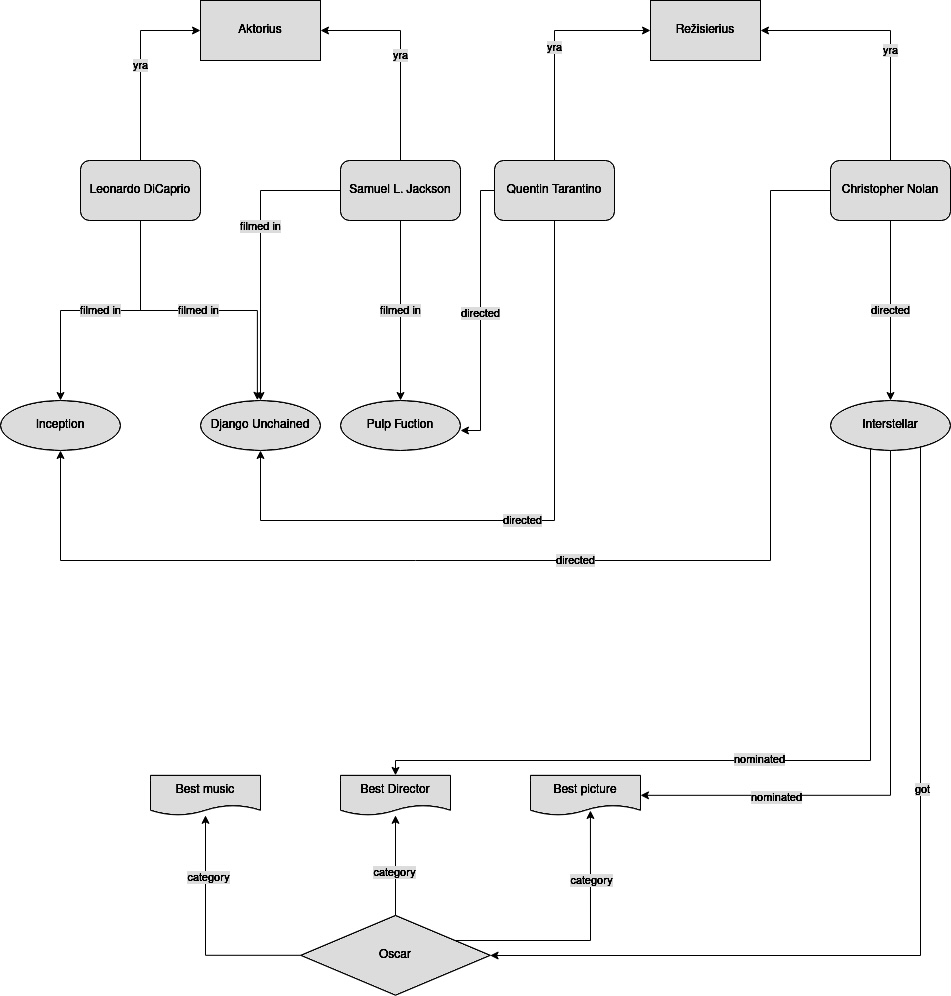
\includegraphics[width=1\textwidth]{img/grafas.jpeg}
  \caption{Žinių grafas}
  \label{fig:sample_image}
\end{figure}
\pagebreak

Klausimai:
\begin{enumerate}
    \item Ar gavo Christopherio Nolano filmas "Interstellar" gavo Oscar už nominacija best picture?
    \item Kokiame filme vaidino Samuel L. Jackson?
    \item Ar Christopherio Nolano filmas "Interstellar" gavo Oscar?
\end{enumerate}

Norint rasti atsakymus į šiuos klausimus, naudojame SPARQL užklausų kalbą. SPARQL užklausos yra parengtos pagal RDF modelį. Taigi gauname tokį RDF modelio kodą:
\begin{lstlisting}[captionpos=b, caption=Pavyzdžio RDF modelis, label=lst:sparql,
   basicstyle=\ttfamily,frame=single]
@prefix rdf: <http://www.w3.org/1999/02/22-rdf-syntax-ns#> .
@prefix rdfs: <http://www.w3.org/2000/01/rdf-schema#> .
@prefix ex: <http://example.com/> .

ex:Aktorius rdf:type rdfs:Class .
ex:Reziserius rdf:type rdfs:Class .
ex:LeonardoDicaprio rdf:type ex:Aktorius .
ex:SamuelLJackson rdf:type ex:Aktorius .
ex:QuentinTarantino rdf:type ex:Reziserius .
ex:ChristopherNolan rdf:type ex:Reziserius .
ex:Inception rdf:type rdfs:Class .
ex:DjangoUnchained rdf:type rdfs:Class .
ex:PulpFiction rdf:type rdfs:Class .
ex:Interstellar rdf:type rdfs:Class .
ex:BestMusic rdf:type rdfs:Class .
ex:BestDirector rdf:type rdfs:Class .
ex:BestPicture rdf:type rdfs:Class .
ex:Oscar rdf:type rdfs:Class .

ex:LeonardoDicaprio ex:filmedIn ex:Inception .
ex:LeonardoDicaprio ex:filmedIn ex:DjangoUnchained .
ex:SamuelLJackson ex:filmedIn ex:DjangoUnchained .
ex:SamuelLJackson ex:filmedIn ex:PulpFiction .
ex:QuentinTarantino ex:directed ex:PulpFiction .
ex:ChristopherNolan ex:directed ex:Inception .
ex:ChristopherNolan ex:directed ex:Interstellar .
ex:Interstellar ex:nominated ex:BestMusic .
ex:Interstellar ex:nominated ex:BestDirector .
ex:Interstellar ex:got ex:Oscar .
ex:Oscar ex:hasCategory ex:BestMusic .
ex:Oscar ex:hasCategory ex:BestDirector .
ex:Oscar ex:hasCategory ex:BestPicture .
\end{lstlisting}
\pagebreak

\begin{figure}[htbp]
  \centering
  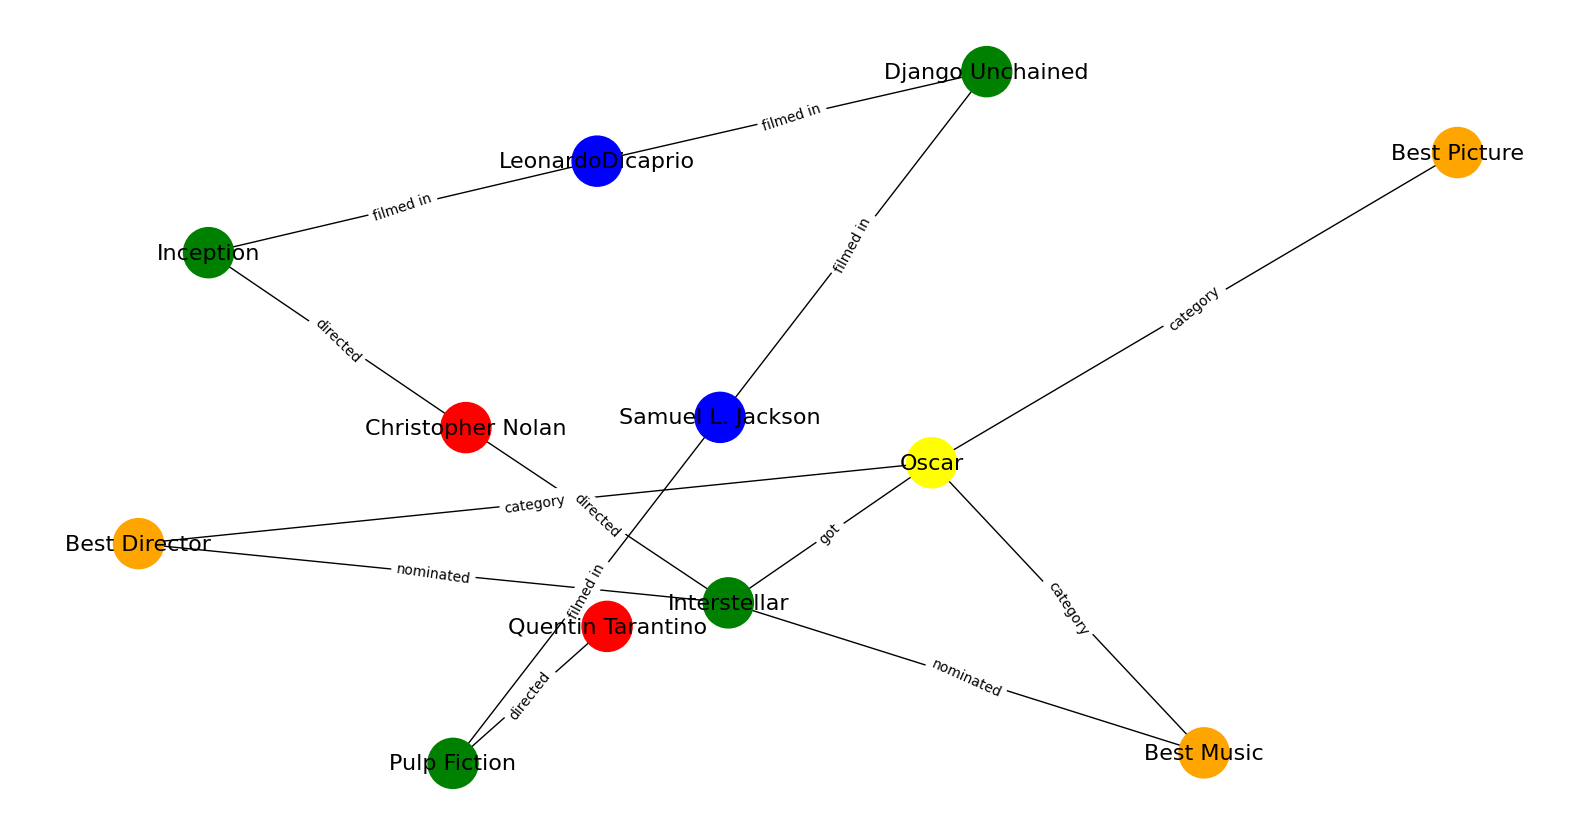
\includegraphics[width=1\textwidth]{img/last_graph_rdf.png}
  \caption{Žinių grafas naudojant python networkX ir Matplotlib biblioteka}
  \label{fig:sample_image}
\end{figure}

\subsection{SPARQL užklausos atsakantys į klausymą ir vykdymo scenarijų analizė}
Ar gavo Christopherio Nolano filmas "Interstellar" gavo Oscar už nominacija best picture?
Galime naudoti tokį užklausą:
\begin{lstlisting}[captionpos=b, caption=Užklausa 1, label=lst:sparql,
   basicstyle=\ttfamily,frame=single]
PREFIX rdf: <http://www.w3.org/1999/02/22-rdf-syntax-ns#>
PREFIX rdfs: <http://www.w3.org/2000/01/rdf-schema#>
PREFIX ex: <http://example.com/>

SELECT ?result WHERE {
  ex:Interstellar ex:got ex:Oscar .
  ex:Oscar ex:hasCategory ex:BestPicture .
  ex:Oscar ex:hasCategory ?result .
}

\end{lstlisting}

Ši užklausa ieško kategorijos BestPicture susiejimo su Oscar, kuris susiejamas su Interstellar. Jei toks susiejimas egzistuoja, užklausa grąžins ?result kintamąjį, kuris bus kategorijos pavadinimas (BestPicture). Jei tokio susiejimo nėra, užklausa grąžins tuščią rezultatų rinkinį.
\pagebreak

Kokiame filme vaidino Samuel L. Jackson?
\begin{lstlisting}[captionpos=b, caption=Užklausa 2, label=lst:sparql,
   basicstyle=\ttfamily,frame=single]
PREFIX rdf: <http://www.w3.org/1999/02/22-rdf-syntax-ns#>
PREFIX ex: <http://example.com/>

SELECT ?filmas
WHERE {
  ex:SamuelLJackson ex:filmedIn ?filmas .
}
\end{lstlisting}

Šiuo atveju mes norime gauti ?filmas kintamąjį, kuris atitiks visus filmus, kuriuose vaidino Samuelis L. Jacksonas.
WHERE frazėje nurodomi kriterijai, pagal kuriuos bus filtruojami RDF duomenys. Šiuo atveju mes ieškome visų ?filmas kintamojo reikšmių, kurios yra susietos su Samuelio L. Jacksono ir kokiu nors filmu ryšiu (naudojant ex:filmedIn savybę).

Ar Christopherio Nolano filmas "Interstellar" gavo Oscar?
\begin{lstlisting}[captionpos=b, caption=Užklausa 3, label=lst:sparql,
   basicstyle=\ttfamily,frame=single]
PREFIX rdf: <http://www.w3.org/1999/02/22-rdf-syntax-ns#>
PREFIX ex: <http://example.com/>

SELECT ?oscar
WHERE {
  ex:Interstellar ex:got ?oscar .
  ?oscar ex:hasCategory ex:BestPicture .
}

\end{lstlisting}
Ši užklausa naudoja ASK formą, kad patikrintų, ar yra atitikmuo tarp ex:Interstellar ex:got ex:Oscar. ir ex:Oscar ex:hasCategory ex:BestPicture. 
Sprendimas grąžins true, jei yra atitikimas ir false, jei nėra.

\sectionnonum{Rezultatai ir išvados}
Išanalizavus šią temą, galime padaryti keletą svarbių išvadų. Žinių grafai yra labai patogus ir efektyvus būdas atvaizduoti ir saugoti duomenis. Naudojant RDF modeli, kaip vieną iš pagrindinių žinių grafų modeliavimo metodų, galima lengvai naudotis SPARQL užklausos kalba. SPARQL, yra universali ir galinga užklausų kalba. Pateikus pavyzdinį žinių grafo aprašymą ir SPARQL užklausų scenarijus, galime matyti, kad SPARQL yra labai intuityvi ir jį galima pritaikyti įvairiems užklausų tipams. 


\printbibliography[heading=bibintoc]



\end{document}
